\documentclass[a4paper, 12pt]{article}
\usepackage[utf8]{inputenc}
\usepackage[brazil]{babel}
\usepackage{amstext} 	% need for \text command
\usepackage{amsmath}    % need for subequations
\usepackage{amssymb}
\usepackage{graphicx}   % need for figures
\usepackage{verbatim}   % useful for program listings
\usepackage{color}      % use if color is used in text
\usepackage{subfigure}  % use for side-by-side figures
\usepackage{hyperref}   % use for hypertext links, including those to external documents and URLs
\usepackage{pictexwd}	% use for pictex graphs
\usepackage{booktabs}	% use for Publication quality tables in LaTeX

%\author{Vítor M. Martins}
\title{PMR2370}

\begin{document}
\maketitle
%\newpage
%\tableofcontents
%\newpage

\section{Engrenagens}
\paragraph{Classificação}
\begin{itemize}
\item Posição dos eixos
\item Formato do Blanck
\item Orientação dos Dentes
\end{itemize}

\[\begin{tabular}{|c|c|c|}
\hline 
Paralelos & Cilíndrico & Reto Helicoidal \\ 
\hline 
Interceptam & Cônico & Reto Helicoidal \\ 
\hline 
Reversos & Hiperbólico Cilíndrico & Helicoidal \\ 
\hline 
\end{tabular} \]

\section{Cinemática}
\subsection{Ação de Perfis Conjugados}
\begin{enumerate}
\item movimento de saída
\item movimento de entrada
\item geometria dos perfis
\end{enumerate}

\paragraph*{Relação de transmissão constante}
\[i=\frac{n_{1}}{n_{2}}\]
\begin{enumerate}
\item motor
\item movido
\end{enumerate}

\begin{figure}[h]
\begin{center}
\includegraphics[scale=0.38]{./fig/Montagem1.jpg}
\caption{\label{fig:1}1} 
\end{center}
\end{figure}

\[\frac{\overline{O_{2}P}}{\overline{O_{1}P}} \ cte\]
\[V_{1}=V_{2}\]
\[\omega _{1}\overline{O_{1}P} = \omega _{2}\overline{O_{2}P}\]
\[\frac{\omega _{1}}{\omega _{2}} = \frac{\overline{O_{2}P}}{\overline{O_{1}P}} = cte \]

Evolvente de círculo: ponto de uma reta que rola sem escorregar sobre uma circunferência de base.
\\
\\
\ \ \ Fabricação $\rightarrow$ Processo de geração
\\

\subsection{Geometria ECDR}

\begin{figure}[h]
\begin{center}
\includegraphics[scale=0.38]{./fig/Montagem2.jpg}
\caption{\label{fig:2}2} 
\end{center}
\end{figure}

p = passo (medido em arco) \\
$\pi d$=z $\times$ p \\
z = nº de dentes \\
d = diâmetro primitivo \\

\[d = z \times \frac{p}{\pi} \]

\begin{equation}
\frac{p}{\pi} = m
\label{eq:1}
\end{equation}
Em que m na equação \ref{eq:1} é o módulo normalizado, referência para todas as dimensões

\begin{equation}
d_{t} = d + 2m
\label{eq:2}
\end{equation}

\begin{equation}
d_{f} = d - 2.5m
\label{eq:3}
\end{equation}

\begin{equation}
h_{z} = 2.25m
\label{eq:4}
\end{equation}

\begin{equation}
f_{r}=0.25m
\label{eq:5}
\end{equation}

\subsection{AGMA (passo diametral)}
Diametral Pitch (EUA)

\paragraph{ECDR}


Em que as equações são:
\begin{itemize}
\item Equaçao \ref{eq:2}: círculo de topo
\item Equaçao \ref{eq:3}: círculo de pé
\item Equaçao \ref{eq:4}: altura do dente
\item Equaçao \ref{eq:5}: folga radial
\end{itemize}

\begin{figure}[h]
\begin{center}
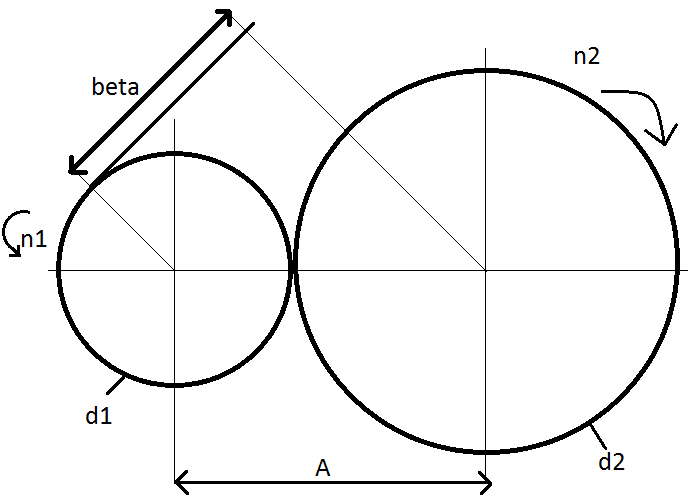
\includegraphics[scale=0.38]{./fig/3.png}
\caption{\label{fig:3}3} 
\end{center}
\end{figure}

\[A = \frac{d_{1}+d_{2}}{2}=\frac{m}{2}(z_{1}+z_{2})\]
\[i = \frac{\omega _{1}}{\omega _{2}} = \frac{d _{1}}{d_{2}}=\frac{z_{1}}{z_{2}}\]

\paragraph{Dente Helicoidal}

\[B_{x}=\frac{B}{\cos \beta}\]
\[10º \leqslant \beta \leqslant 30º\]

\begin{figure}[h]
\begin{center}
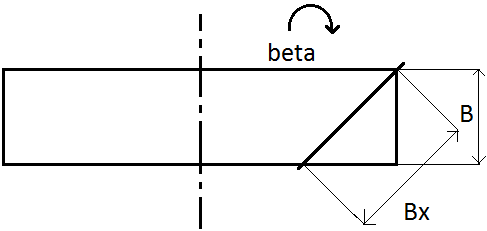
\includegraphics[scale=0.48]{./fig/4.png}
\caption{\label{fig:4}4} 
\end{center}
\end{figure}

\begin{figure}[h]
\begin{center}
\includegraphics[scale=0.21]{./fig/Montagem3.jpg}
\caption{\label{fig:4}frontal} 
\end{center}
\end{figure}

\[p_{f}=\frac{p_{n}}{\cos (\beta)}\]

\[d = \frac{p_{f}}{\pi} \footnote{$m_{f}$}  \times z  = \frac{p_{n}}{\pi \cos (\beta)} \footnote{m} \times z  \] 


\begin{figure}[h]
\begin{center}
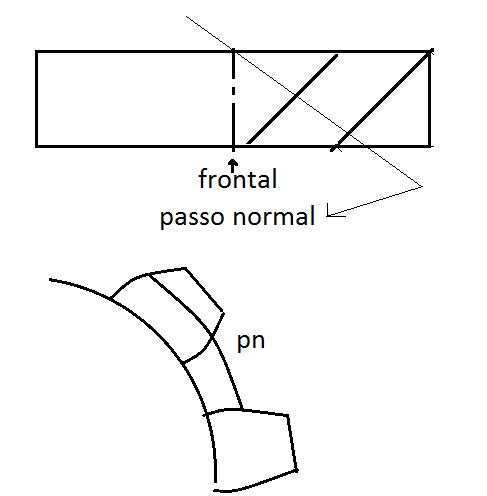
\includegraphics[scale=0.48]{./fig/5.png}
\caption{\label{fig:6}6} 
\end{center}
\end{figure}

\[d = \frac{m}{cos \beta} \times z\]
\[A = \frac{d_{1}+d_{2}}{2}=\frac{m}{2}\frac{z_{1}+z_{2}}{\cos \beta}\]

\begin{figure}[h]
\begin{center}
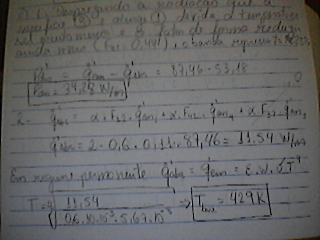
\includegraphics[scale=0.48]{./fig/6.png}
\caption{\label{fig:7}7} 
\end{center}
\end{figure}

\newpage

\subsection{Forças ECDR}

Para evolvente:
\begin{itemize}
\item $\alpha$ constante $\rightarrow$ ângulo de pressão ($\alpha$ = 20º)
\item $F_{e}$ = Força de Engrenamento normal ao dente no ponto de contato
\item $F_{t}$ = força tangencial
\item $M_{t}$ = torque
\end{itemize}

\[F_{t}=\frac{2M_{t}}{d}\]
\[F_{r}=F_{t} \tan \alpha\]
\[F_{e}= \frac{F_{t}}{\cos \alpha}\]

\begin{figure}[h]
\begin{center}
\includegraphics[scale=0.2]{./fig/Montagem4.jpg}
\caption{\label{fig:8}8} 
\end{center}
\end{figure}

\pagebreak

\subsection{Dente Helicoidal}

\[F_{t} = \frac{2M_{t}}{d}\]
\[F_{e} = \frac{F_{t}}{\cos (\alpha) \cos (\beta)}\]
\[F_{a}=F_{t} \tan \beta\]
\[F_{r}= \frac{F_{t} \tan \alpha}{\cos \beta}\]

\begin{figure}[h]
\begin{center}
\includegraphics[scale=0.24]{./fig/Montagem5.jpg}
\caption{\label{fig:9}9} 
\end{center}
\end{figure}

\paragraph{Eixos Reversos}

\begin{figure}[h]
\begin{center}
\includegraphics[scale=0.2]{./fig/7.png}
\caption{\label{fig:10}Não é classificado como engrenagem} 
\end{center}
\end{figure}

\pagebreak

\subsection{Engrenagens Cônicas}

\begin{figure}[h]
\begin{center}
\includegraphics[scale=0.4]{./fig/8.png}
\caption{\label{fig:11}11} 
\end{center}
\end{figure}

\[\sigma _{i} + \sigma _{e} = \sigma \footnote{ângulo entre eixos} \] 
\subparagraph{ECDR}
\[F_{e} = \frac{F_{t}}{\cos (\alpha _{0})} \left\{ 
\begin{array}{c}
\sin \alpha _{i} \\
\sin \sigma _{i} \\
\sin \alpha _{0} \\
\cos \sigma _{1} 
\end{array} \right.
\]

\[F_{r} = F_{e} \tan (\alpha) \sin (\sigma _{1})\]
\[F_{a} = F_{t} \tan \alpha \cos \sigma _{i}\]

\[\sigma _{max} = \frac{M}{I} \frac{h}{2}\]
\[M = F_{t} \times h_{z}\]
\[I = \frac{B h_{b}^{3}}{12}\]

\[\sigma = \frac{6 F_{t} \times h_{z}}{B h_{b}^{2}}\]

\paragraph*{cremalheira}

\[\frac{h_{z}}{h_{b}/2}=\frac{h_{b}/2}{x}\]
\[x = \frac{h_{b}^{2}}{4 h_{z}}\]
\[\sigma = \frac{F_{t}}{Bx*\frac{2}{3}}\times\frac{m}{m}\]

\begin{equation}
y = \frac{2x}{3m}
\label{eq:6}
\end{equation}
Em que \ref{eq:6} representa o fator de forma de Levis ($\alpha,z$) (tabelado)

\begin{equation}
\sigma = \frac{F_{t}}{B \times m \times y}
\label{eq:7}
\end{equation}
Em que \ref{eq:7} é estática ou muito lenta

\begin{figure}[h]
\begin{center}
\includegraphics[scale=0.4]{./fig/9.png}
\caption{\label{fig:12}12} 
\end{center}
\end{figure}

\subsection{Fator de aplicação rápida de forma $K_{\upsilon}$ (Berth)}
$v$ = m/s (AGMA)
\begin{equation}
K_{\upsilon}=\frac{6.1+v}{6.1}
\label{eq:8}
\end{equation}
Equaçao \ref{eq:8} representa $K_{\upsilon}$ para dentes usinados com fresa módulo

\begin{equation}
K_{\upsilon}=\frac{3.56+\sqrt{v}}{3.56}
\label{eq:9}
\end{equation}
Equação \ref{eq:9} representa $K_{\upsilon}$ para dentes usinados por geração

\begin{equation}
K_{\upsilon}=\sqrt{ \frac{5.56+\sqrt{v}}{5.56} }
\label{eq:10}
\end{equation}
Equação \ref{eq:10} representa $K_{\upsilon}$ para dentes retificados.

\subparagraph*{$K_{s}$  =fatores de serviço (AGMA)}
\[\sigma = \frac{(K_{s}\ ou\ K_{\upsilon}) \times F_{t}}{B \times m \times y} \leqslant \sigma _{fp}\]

\subsection{Contato (Hertz $\sim$ 1880)}

\begin{figure}[h]
\begin{center}
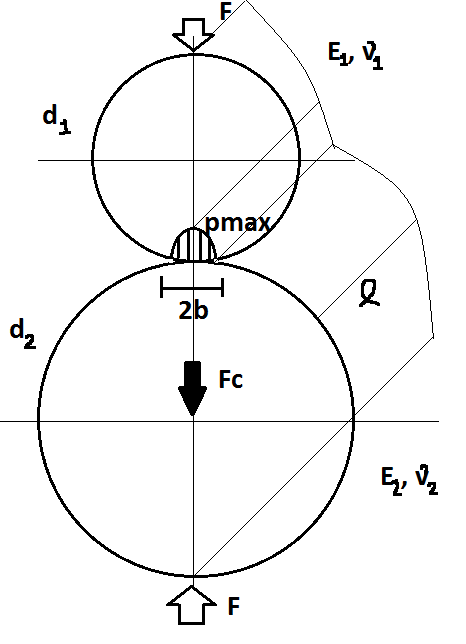
\includegraphics[scale=0.4]{./fig/10.png}
\caption{\label{fig:13}13} 
\end{center}
\end{figure}

\[p_{max} = \frac{2F}{\pi \times b \times l}\]
\[
b^{2} = \left\{    \frac{2F}{\pi l} \frac{[(1-\upsilon_{1}^{2})/E_{1}]+[(1-\upsilon_{2}^{2})/E_{2}]}{(1/d_{1})+(1/d_{2})}     \right\}\]

\[p_{max}^{2}=\frac{4F^{2}}{\pi ^{2} \times b^{2} \times l^{2}}\]

\[p_{max}^{2}=\frac{4F}{\pi ^{2} l^{2}} \frac{ \pi l}{2F} \frac{(1/d_{1})+(1/d_{2})}{[(1-\upsilon_{1}^{2})/E_{1}]+[(1-\upsilon_{2}^{2})/E_{2}]}\]

\[p_{max}^{2}=\frac{2F}{\pi l} \times \frac{(1/d_{1})+(1/d_{2})}{[(1-\upsilon_{1}^{2})/E_{1}]+[(1-\upsilon_{2}^{2})/E_{2}]}\]

\begin{figure}[h]
\begin{center}
\includegraphics[scale=0.25]{./fig/Montagem6.jpg}
\caption{\label{fig:14}14} 
\end{center}
\end{figure}

l = B

\[F = \frac{F_{t}}{\cos \phi}\]
\[F_{t} = \frac{2M_{t}}{d_{\rho}}\]
\[d_{1}=2\rho _{1}\]
\[d_{2}=2\rho _{2}\]

\subparagraph*{Curva Evolvente}
\[\rho _{1} = \frac{d_{\rho 1}\footnote{diâmetro primitivo}}{2} \sin \alpha \]
\[\rho _{2} = \frac{d_{\rho 2}}{2} \sin \alpha \]

\subparagraph*{Engrenagem:}

\[p_{max}^{2}=\frac{2 F_{t}}{\pi (\cos (\alpha))B} \times \frac{(1/d_{\rho 1}\sin \alpha)+(1/d_{\rho 2}\sin \alpha)}{[(1-\upsilon_{1}^{2})/E_{1}]+[(1-\upsilon_{2}^{2})/E_{2}]}\]

Seja: 

\[C_{p}^{2} = \frac{1}{\pi \left(  \frac{1-\upsilon_{1}^{2}}{E_{1}} + \frac{1-\upsilon_{2}^{2}}{E_{2}}  \right) }\]

depende apenas das propriedades dos materiais.
Lembrando que:
\[i = \frac{d_{\rho 2}}{d_{\rho 1}}\]
Temos:
\[
\frac{1}{d_{\rho 1}\sin \alpha} + \frac{1}{d_{\rho 2}\sin \alpha} = \frac{1}{\sin \alpha} \left(  \frac{1}{d_{\rho 1}} + \frac{1}{d_{\rho 2}}  \right) = \frac{1}{d_{\rho 1}\sin \alpha} \left(  1 + \frac{1}{i}  \right) \]

\[p_{max}^{2}=C_{p}^{2}\frac{2F_{r}}{B\cos \alpha} \frac{1}{d_{\rho 1} \sin \alpha} \left( \frac{i+1}{i}  \right)\]

\[p_{max}^{2}=C_{p}^{2}\frac{2}{\cos \alpha \sin \alpha} \frac{F_{r}}{B d_{\rho 1} } \left( \frac{i+1}{i}  \right)\]

\[F_{t} = \frac{2M_{t1}}{d_{\rho 1}}\]

\[p_{max}^{2}=C_{p}^{2}\frac{4}{\cos \alpha \sin \alpha} \frac{M_{t}}{B d_{\rho 1}^{2} } \left( \frac{i+1}{i}  \right)\]
Volume do Pinhão:

\[ B d_{\rho 1}^{2} =C_{p}^{2}\frac{4}{\cos \alpha \sin \alpha} \frac{M_{t}}{ \overline{p_{max}^{2}} } \left( \frac{i+1}{i}  \right)\]

$\overline{p_{max}^{2}}$ = pressão limite
\\
\\
Contato é mais crítico em rotações maiores (acima de 100 rpm) em engrenagens lentas, é crítica flexão na base.

\begin{figure}[h]
\begin{center}
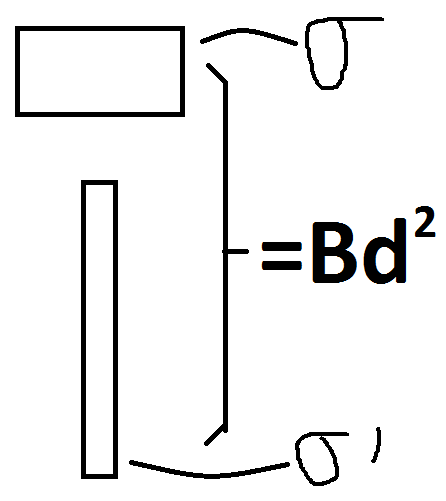
\includegraphics[scale=0.35]{./fig/11.png}
\caption{\label{fig:15}15} 
\end{center}
\end{figure}





\end{document}